
%% This work may be distributed and/or modified under the
%% conditions of the LaTeX Project Public License, either version 1.3
%% of this license or (at your option) any later version.
%% The latest version of this license is in
%%   http://www.latex-project.org/lppl.txt
%% and version 1.3 or later is part of all distributions of LaTeX
%% version 2005/12/01 or later.
%% 
%% This work has the LPPL maintenance status `maintained'.
%% 
%% The Current Maintainer of this work is Liam Huang.
%% 
\documentclass{mcmthesis}
\mcmsetup{CTeX = false,   % 使用 CTeX 套装时,设置为 true
        tcn = 56074, problem = D,
        sheet = true, titleinsheet = true, keywordsinsheet = true,
        titlepage = false, abstract = true}
\usepackage{times}
\usepackage{lipsum}
\usepackage{amsmath}
\usepackage{indentfirst}


\title{How to optimize passenger throughout}
\author{Dingcheng Guo \\ Yuchen Lu \\ Jiawen Wu}
%\author{\small \href{http://www.baidu.com/}
 %{\includegraphics[width=7cm]{mcmthesis-logo}}}
\date{\today}
\begin{document}
\numberwithin{equation}{section}
\begin{abstract}

\begin{keywords}
keyword1; keyword2;keyword3%
\end{keywords}
\end{abstract}

\maketitle
\section{Introduction}%1
\subsection{Background}%1.1
Following the terrorist attacks in the US on September 11, 2001, airport security has been significantly enhanced throughout the world. Airports have security checkpoints, where passengers and their baggage are screened for explosives and other dangerous items. The objectives of these security measures are to prevent passengers from hijacking or destroying aircraft and to keep all passengers safe during their travel. However, airlines have a vested interest in maintaining a positive flying experience for passengers by minimizing the time they spend waiting in line at a security checkpoint and waiting for their flight. Therefore, there is a tension between desires to maximize security and minimizing inconvenience to passengers.

In 2016, the U.S. Transportation Security Agency (TSA) came under sharp criticism for extremely long lines, in particular at Chicago's O'Hare international airport. Following this public attention, the TSA invested in several modifications to their checkpoint equipments and procedures and increased staffing in the more highly congested airports. While these modifications were somewhat successful in reducing waiting times, no one konws how much cost the TSA incurred to implement the new measures and increase staffing. In addition to the issues at O'Hare, there have also been accidents of unexplained and unpredicted long lines at other airports, including airports that normally have short wait times. This high variance in checkpoint lines can be extremely costly to passengers as they decide between arriving unnecessarily early or potentially missing their scheduled flight. 



\emph{center of percussion} [Brody 1986]

\begin{Theorem} \label{thm:latex}
\LaTeX
\end{Theorem}
\begin{Lemma} \label{thm:tex}
\TeX .
\end{Lemma}
\begin{proof}
The proof of theorem.
\end{proof}

\subsection{Other Assumptions}%1.2

\begin{itemize}
\item
\item
\item
\item
\end{itemize}



\section{Analysis of the Problem}%2
\begin{figure}[h]
\small
\centering
\includegraphics[width=12cm]{mcmthesis-aaa.eps}
\caption{aa} \label{fig:aa}
\end{figure}


\begin{equation}
\frac{dy}{dx}=ax \label{aa}
\end{equation}
from \eqref{aa} we have

\[
  p_{j}=\begin{cases} 0,&\text{if $j$ is odd}\\
  r!\,(-1)^{j/2},&\text{if $j$ is even}
  \end{cases}
\]


\section{Calculating and Simplifying the Model}%3
\subsection{The current process for a US airport security checkpoint}
\begin{figure}[htbp]
  \centering
  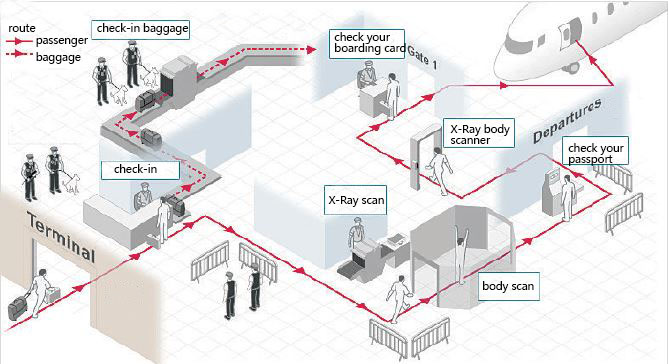
\includegraphics[width=0.85\textwidth]{airport.jpg}
  \caption{Airport}\label{fig:digit}
\end{figure}

\subsection{The Analysis of The Passengers Queueing Theory}
		Since the arrival of the passengers and the sercuity check for every passengers is random, the passenger sercuity check system is a typically random service system. This system has the following characteristics:
			\begin {enumerate}
				\item Those who need sercuity check are those who want to get aboard. The number of passengers are infinite. The arrival time of each passenger is independent and the distribution of service time is also random.
				\item Zone A, Zone B and Zone C can be regarded as servers of this system. The servivce time for each passenger is independent.
				\item The service discipline in this system is ``First in first out'', which states that customers are served one at a time and that the customer that has been waiting the longest is served first.
			\end{enumerate}
\subsection{System Model Assumption}%3.2
Before we obtain the model assumption, we need to determine which distribution the system input and service process subject to. We assume the theoretical distributions of system input and service process are Poission Distribution and Negative Exponential Distribution.
\subsubsection{ Poission  Distribution}
we set $ N(t) $ to represent the number of passengers'  arrival in $ [0,t)(t>0) $ and $ P_n(t_1,t_2) $
to represent the probability of $ n(n\geqslant 0) $ passengers'  arrival  in $ [t_1,t_2)(t_2>t_1) $. Hence,we obtain,

\begin{equation}
P_n(t_1,t_2)=P\{  N(t_2)-N(t_1) =n \} \qquad (t_2>t_1,n\geqslant 0)
\end{equation}

when $P_n(t_1,t_2)$ satisfies the following three conditions, we think the passengers'  arrival subject to Poisson distribution.
\par 1)Passengers arrive at different times independent of each other.
\par 2)For sufficiently small $\Delta t$, the probability of a passenger arrive at $[t,t+\Delta t)$ is independent of $t$ and proportional to the length of the interval  $\Delta t$.
Thus, we have,

\begin{equation}
P_1(t,t+\Delta t)=\lambda \Delta t+o(\Delta t)  \label{e2}
\end{equation}

in where $o(\Delta t)$ means the high order infinitesimal of $\Delta t$ as $\Delta t \rightarrow 0$
\par 3)For sufficiently small $\Delta t$, the probability of two or more  passengers arrive at $[t,t+\Delta t)$ is so small that could be ignored. Then we abtain,
 
\begin{equation}  
\sum\limits_{n=2}^\infty P_n(t,t+\Delta t)=o(\Delta t)   \label{e3}
\end{equation}

From equations \eqref{e2} and  \eqref{e3} we have the probability of the  passengers don't arrive at $[t,t+\Delta t)$ is shown as below.

\begin{equation}
P_0(t,t+\Delta t)=1-\lambda \Delta t+o(\Delta t)
\end{equation}


If the process of input is Poission manifold,then we have,

\begin{equation}
P_n(t,t+\Delta t)=P_n(t)(1-\lambda \Delta t)+P_{n-1}(t)\lambda \Delta t+o(\Delta t) \label{e5}
\end{equation}

Let  $\Delta t \rightarrow 0$. By combining \eqref{e5} and initial condition, we have,

\begin{equation}    \label{e6}
\left\{
       \begin{array}{lr}
           \frac {d P_n(t)}{d t}=-\lambda P_n(t)+\lambda P_{n-1}(t)\qquad n\geqslant 1\\
            P_n(0)=0
        \end{array}
\right.
\end{equation}

when$n=0$,we have,
\begin{equation}    \label{e7}
\left\{
       \begin{array}{lr}
           \frac {d P_0(t)}{d t}=-\lambda P_0(t)\\
            P_0(0)=1
        \end{array}
\right.
\end{equation}


By solving equations \eqref{e6} and \eqref{e7} ,we get,
\begin{equation}
 P_n(t)=\frac{(\lambda t)^n}{n!} e^{-\lambda t}\qquad t>0\, , n=0,1,2,\cdots
\end{equation}


\subsubsection{Negative Exponential Distribution}
If the probability density function of random variables T is shown as below.
\begin{equation}    
f_T(t)=\left  \{
       \begin{array}{lr}
           \lambda e^{-\lambda t}\qquad t\geqslant 0\\
            0\qquad\qquad t<0
        \end{array}
\right.
\end{equation}


Hence T subject to negative exponential distribution and the function of distribution is written as follow.

\begin{equation}    
F_T(t)=\left  \{
       \begin{array}{lr}
          1- \lambda e^{-\lambda t}\qquad\,  t\geqslant 0\\
            0\qquad\qquad\qquad t<0
        \end{array}
\right.
\end{equation}

when the  process of input is Poission manifold, the interval of passengers' arrival T subject to  negative exponential distribution. As for Poission  distribution, at least one passenger arrives at $[0,t)$  probability can  be written as


\begin{equation}
1-P_0(t)=1-e^{-\lambda t}\qquad t>0
\end{equation}
which can be rewritten as
\begin{equation}
 P\{T\leqslant t \}=F_T(t)
\end{equation}


Hence, the time of arrival of passengers is independent of each other and is a negative exponential distribution.The input process is equivalent to the Poisson distribution.

	Based on the basic knowledgee about the queueing theory, we can make these assumptions about the passengers queueing model.
		\begin{enumerate}
			\item Arrival process
			
			 The arrival of passengers are random, and successive customers arrive after intervals which independently are exponentially distributed. So we assume that the arrival of pessagers is subject to a Poisson distribution with the average arrival rate ${\lambda}$.
			\item The behavior of passengers 
			
			 We assume that passengers are patient and willing to wait for a long time.
			\item The service discipline 
			
			 Passengers will be served one by one when taking sercurity check. We have various scheduling policies that can be used in this situation and we choose ``First in first out'' ,which is most commonly used in our daily life, as our principle.
			\item The service capacity 
			
			 In the sercuity checkpoints, we find that Zone A is a system where there exist only one server, and Zone B and Zone C are the systems with a group of servers helping the passengers.
		\end{enumerate}	
		
	So, we assume that the sercurity checkpoint is such a system consisting of a subsystem with only one server, called M/M/1 queue, and another subsystem with several servers, called M/M/c queue.

	\subsection{Model of The Arrival of Pasengers} \label{flag1.1} %3.3
		Maximum likelihood estimation (MLE) is a method of estimating the parameters of a statistical model given observations, by finding the parameter values that maximize the likelihood of making the observations given the parameters. 

		Suppose there is a sample ${X_1,X_2,\dots,X_n}$ for which the probability density (or mass) function of each ${X_i}$ is ${f(x_i;\theta)}$.  Then, the joint probability mass (or density) function of ${X_1,X_2,\dots,X_n}$, which we'll call ${L(\theta)}$ is:
			\begin{gather}
				L( \theta) = P(X_1 = x_1, X_2 = x_2, \dots, X_n = x_n) \notag \\
				= f(x_1; \theta)\cdot f(x_2; \theta) \cdots f(x_n; \theta) = \prod_{i=1}^{n}f(x_i; \theta) \label{flag1}
			\end{gather}
		The first equality is of course just the definition of the joint probability mass function. The second equality comes from that fact that we have a random sample, which implies by definition that the ${X_i}$ are independent.And, the last equality just uses the shorthand mathematical notation of a product of indexed terms. Now, in light of the basic idea of maximum likelihood estimation, one reasonable way to proceed is to treat the "likelihood function" ${L(\theta)}$ as a function of ${\theta}$, and find the value of ${\theta}$ that maximizes it.

		In practice the algebra is often more convenient when working with the natural logarithm of the likelihood function, called the log-likelihood:
			\begin{equation}
				\ln L(\theta) = \sum_{i=1}^{n}\ln f(x_i;\theta). 
			\end{equation}
		Take the partial derivative of the log likelihood with respect to ${\theta}$, and set to 0 to solve for ${\hat \theta}$. And ${\hat \theta}$ is maximum likelihood estimator.

		In this reserach, we assume that the arrival of passengers are subject to Poisson distribution. First, we use Maximum likelihood estimation to estimate the parameter ${\lambda}$.

		We assume that the sample ${X}$ is subject to Poisson distribution with the rate parameter ${\lambda}$, or
			\begin{equation}
				P(X = i) = \frac {\lambda ^ i}{i!}e^{-\lambda},i=0,1,2,\dots
			\end{equation}
		${X_1,X_2, \dots ,X_n}$ are samples coming from overall sample ${X}$, and ${x_1,x_2, \dots ,x_n}$ are values corresponding to the samples  ${X_1,X_2, \dots ,X_n}$. 
		From equation \eqref{flag1}, we can get the likelihood function L(p) is, by definition:
			\begin{equation}
				L(\theta) = \prod_{i=1}^{n}P(X=x_i) = \prod_{i=1}^{n} {\frac{{\lambda}^x_i}{x_i!}}e^{-\lambda}
			\end{equation}
		By taking  the natural logarithm of the likelihood function above, then
			$${\ln L(\lambda) = \ln {\lambda} \cdot \sum_{i=1}^{n}x_i-n\lambda- \sum_{i=1}^{n}\ln (x_i!)}$$
		Take the partial derivative of the log likelihood with respect to ${\lambda}$,we obtain
			$${\frac {d \ln L(\lambda)}{d \lambda} = \frac {\sum\limits_{i=1}^{n}x_i}{\lambda} -n}$$
		Let the equation above equal to zero, we get
			\begin{equation}
				\hat \lambda = \frac{1}{n} \sum_{i=1}^{n}x_i = \overline x
 			\end{equation}
		Hence, the  maximum likelihood estimator is
			\begin{equation}
				\hat \lambda = \frac{1}{n} \sum_{i=1}^{n}X_i = \overline X
			\end{equation}
	\subsection{Models of the sercurity check system}%3.4
		\subsubsection{M/M/1 Queue}
			The M/M/1 queue is a simple model where a single server serves jobs that arrive according to a Poisson process and have exponentially distributed service requirements. 
			
			Let ${E}$ represnt the number of times of entering state ${n}$, and ${L}$ represent the number of times of leaving state ${n}$. We have ${|E - L| \in \{0,1\}}$. When the system arrives at steady state, which means ${t}$, we have, therefore arrival rate = removed rate.
			
			Hence, the balance equation of this system is 
				\begin{equation}    
					\left  \{
       						\begin{array}{lr}
        						   - \lambda _0 P_0 + \mu _1 P_1 = 0\\
        						   \lambda _{n-1} P_{n-1} + \mu _{n+1} P_{n+1} -(\lambda _n + \mu _n ) P_n = 0,n>1
  					      \end{array}
					\right.
				\end{equation}
			By balance equation, 
			$${P_1 = \frac{\lambda _0}{ \mu _1}P_0 }$$
			By mathematical induction,
				\begin{equation}
					P_n = \frac {\lambda _{n-1} \lambda _{n-2} \dots \lambda_0}{\mu _n \mu_{n-1} \dots \mu _1}P_0 = P_0\prod_{i=0}^{n-1} \frac{\lambda _i}{\mu _{i+1}}
				\end{equation}
			Since ${\sum\limits_{n=0}^{ \infty } P_n = 1}$, we get
				\begin{equation}
					P_0 = \frac{1}{1 + \sum\limits_{n=1}^{ \infty} \frac {\lambda _{n-1} \lambda _{n-2} \dots \lambda_0}{\mu _n \mu_{n-1} \dots \mu _1}}
				\end{equation}
				
			From \ref{flag1.1} , arrivals occur at rate ${\lambda}$ according to a Poisson process and move the process from state ${i}$ to ${i + 1}$. Service times have an exponential distribution with rate parameter ${\mu}$ in the M/M/1 queue, where ${\frac{1}{\mu}}$ is the mean service time. Arrivals and service times are independent.
			
			We focus on the zone A first. This queueing service system belongs to M/M/1 quequeing, where we obtain
				\begin{equation}    
					\left  \{
       						\begin{array}{lr}
        						  \lambda_i = \lambda\\
        						  \mu_k = \mu
  					      \end{array}
					\right.
				\end{equation}
			We write ${\rho = \frac{\lambda}{\mu}}$ for the utilization of the buffer and  ${\rho}$ represents the average proportion of time which the server is occupied.
			
			So that the probability that the stationary process is in state ${i}$ (contains ${i}$ customers, including those in service) is
			\begin{equation}
			 	P_n = \rho ^n P_0.
			\end{equation}
			Thus the average number of passengers in the system and the average number of waiting paseengers are
				\begin{equation}    
					\left  \{
       						\begin{array}{lr}
			 				L_q = \frac {\rho ^2}{1-\rho}\\
							L_s = \frac{\rho}{1 - \rho}
  					      \end{array}
					\right.
				\end{equation}
			The average response time and the the average time spent waiting are
				\begin{equation}    
					\left  \{
       						\begin{array}{lr}
       							W_s = \frac{1}{\mu - \lambda}\\
       							W_q = \frac{\lambda}{\mu (\mu - \lambda)}
  					      \end{array}
					\right.
				\end{equation}

\subsubsection{M/M/c queue }
Now we set there are c$(c\geqslant 2)$ windows work independently. Passengers would like  to go to the free windows. If there are all busy,than wait until there is a free window.
In M/M/c ,we have 
 

\begin{equation}    
\left  \{
       \begin{array}{lr}
         \lambda_i=\lambda  \qquad \qquad i\geqslant 0\\
           \mu_i=\left  \{
       \begin{array}{lr}
         i\mu  \qquad\, i=1,2,\cdots\\
            c\mu\qquad\, i=n+1,n+2,\cdots
        \end{array}
\right.
        \end{array}
\right.
\end{equation}

We define $\rho=\frac{\lambda}{\mu}$, $\rho_c=\frac{\lambda}{c\mu}$,then we get,
\\stationary distribution probability is shown as below

\begin{equation}    
\left  \{
       \begin{array}{lr}
           P_0=[\sum\limits_{k=0}^{c-1}\frac{1}{k!}\rho ^k+\frac{1}{c!}\frac{1}{1-\rho}\rho ^c]^{-1}\\
            P_n=\frac{\rho ^c}{c!(1-\rho_c)}P_0
        \end{array}
\right.
\end{equation}


The average number of passengers in the system and the average number of waitting passengers can write as
\begin{equation}    
\left  \{
       \begin{array}{lr}
           L_s=\frac{\rho ^2\rho_c}{c!(1-\rho_c)^2}P_0 +\rho \\
          L_q=\frac{\rho ^2\rho_c}{c!(1-\rho_c)^2}P_0 
        \end{array}
\right.
\end{equation}

The average waitting time and average time spend waitting can be written as
\begin{equation}    
\left  \{
       \begin{array}{lr}
           W_s=\frac{\rho ^2\rho_c}{c!(1-\rho_c)^2}P_0 +\rho \\
          W_q=\frac{\rho ^2\rho_c}{c!(1-\rho_c)^2}P_0 
        \end{array}
\right.
\end{equation}



\section{The Model Results}%4


\section{Validating the Model}%5

\section{Conclusions}%6


\section{A Summary}%7

\section{Evaluate of the Mode}%8

\section{Strengths and Weaknesses}%9

\subsection{Strengths}
\begin{itemize}
\item \textbf{Applies widely}\\
This  system can be used for many types of airplanes, and it also
solves the interference during  the procedure of the boarding
airplane,as described above we can get to the  optimization
boarding time.We also know that all the service is automate.
\item \textbf{Improve the quality of the airport service}\\
Balancing the cost of the cost and the benefit, it will bring in
more convenient  for airport and passengers.It also saves many
human resources for the airline. 
\item \textbf{}
\end{itemize}

\subsection{Weaknesses}
\begin{itemize}
\item \textbf{Lack of data}\\
This  system can be used for many types of airplanes, and it also
solves the interference during  the procedure of the boarding
airplane,as described above we can get to the  optimization
boarding time.We also know that all the service is automate.
\item \textbf{Not completely achievable}\\
Balancing the cost of the cost and the benefit, it will bring in
more convenient  for airport and passengers.It also saves many
human resources for the airline. 
\end{itemize}

\begin{thebibliography}{99}
\bibitem{1} D.~E. KNUTH   The \TeX{}book  the American
Mathematical Society and Addison-Wesley
Publishing Company , 1984-1986.
\bibitem{2}Lamport, Leslie,  \LaTeX{}: `` A Document Preparation System '',
Addison-Wesley Publishing Company, 1986.
\bibitem{3}\url{http://www.latexstudio.net/}
\bibitem{4}\url{http://www.chinatex.org/}
\end{thebibliography}


\end{document}

%% 
%% This work consists of these files mcmthesis.dtx,
%%                                   figures/ and
%%                                   code/,
%% and the derived files             mcmthesis.cls,
%%                                   mcmthesis-demo.tex,
%%                                   README,
%%                                   LICENSE,
%%                                   mcmthesis.pdf and
%%                                   mcmthesis-demo.pdf.
%%
%% End of file `mcmthesis-demo.tex'.
